% Options for packages loaded elsewhere
\PassOptionsToPackage{unicode}{hyperref}
\PassOptionsToPackage{hyphens}{url}
%
\documentclass[
  ignorenonframetext,
]{beamer}
\usepackage{pgfpages}
\setbeamertemplate{caption}[numbered]
\setbeamertemplate{caption label separator}{: }
\setbeamercolor{caption name}{fg=normal text.fg}
\beamertemplatenavigationsymbolsempty
% Prevent slide breaks in the middle of a paragraph
\widowpenalties 1 10000
\raggedbottom
\setbeamertemplate{part page}{
  \centering
  \begin{beamercolorbox}[sep=16pt,center]{part title}
    \usebeamerfont{part title}\insertpart\par
  \end{beamercolorbox}
}
\setbeamertemplate{section page}{
  \centering
  \begin{beamercolorbox}[sep=12pt,center]{part title}
    \usebeamerfont{section title}\insertsection\par
  \end{beamercolorbox}
}
\setbeamertemplate{subsection page}{
  \centering
  \begin{beamercolorbox}[sep=8pt,center]{part title}
    \usebeamerfont{subsection title}\insertsubsection\par
  \end{beamercolorbox}
}
\AtBeginPart{
  \frame{\partpage}
}
\AtBeginSection{
  \ifbibliography
  \else
    \frame{\sectionpage}
  \fi
}
\AtBeginSubsection{
  \frame{\subsectionpage}
}
\usepackage{amsmath,amssymb}
\usepackage{lmodern}
\usepackage{iftex}
\ifPDFTeX
  \usepackage[T1]{fontenc}
  \usepackage[utf8]{inputenc}
  \usepackage{textcomp} % provide euro and other symbols
\else % if luatex or xetex
  \usepackage{unicode-math}
  \defaultfontfeatures{Scale=MatchLowercase}
  \defaultfontfeatures[\rmfamily]{Ligatures=TeX,Scale=1}
\fi
\usetheme[]{Luebeck}
% Use upquote if available, for straight quotes in verbatim environments
\IfFileExists{upquote.sty}{\usepackage{upquote}}{}
\IfFileExists{microtype.sty}{% use microtype if available
  \usepackage[]{microtype}
  \UseMicrotypeSet[protrusion]{basicmath} % disable protrusion for tt fonts
}{}
\makeatletter
\@ifundefined{KOMAClassName}{% if non-KOMA class
  \IfFileExists{parskip.sty}{%
    \usepackage{parskip}
  }{% else
    \setlength{\parindent}{0pt}
    \setlength{\parskip}{6pt plus 2pt minus 1pt}}
}{% if KOMA class
  \KOMAoptions{parskip=half}}
\makeatother
\usepackage{xcolor}
\newif\ifbibliography
\usepackage{graphicx}
\makeatletter
\def\maxwidth{\ifdim\Gin@nat@width>\linewidth\linewidth\else\Gin@nat@width\fi}
\def\maxheight{\ifdim\Gin@nat@height>\textheight\textheight\else\Gin@nat@height\fi}
\makeatother
% Scale images if necessary, so that they will not overflow the page
% margins by default, and it is still possible to overwrite the defaults
% using explicit options in \includegraphics[width, height, ...]{}
\setkeys{Gin}{width=\maxwidth,height=\maxheight,keepaspectratio}
% Set default figure placement to htbp
\makeatletter
\def\fps@figure{htbp}
\makeatother
\setlength{\emergencystretch}{3em} % prevent overfull lines
\providecommand{\tightlist}{%
  \setlength{\itemsep}{0pt}\setlength{\parskip}{0pt}}
\setcounter{secnumdepth}{-\maxdimen} % remove section numbering
\usepackage{animate}
\ifLuaTeX
  \usepackage{selnolig}  % disable illegal ligatures
\fi
\IfFileExists{bookmark.sty}{\usepackage{bookmark}}{\usepackage{hyperref}}
\IfFileExists{xurl.sty}{\usepackage{xurl}}{} % add URL line breaks if available
\urlstyle{same} % disable monospaced font for URLs
\hypersetup{
  pdftitle={Probabilistic Programming with STAN},
  pdfauthor={Forrest Koch},
  hidelinks,
  pdfcreator={LaTeX via pandoc}}

\title{Probabilistic Programming with STAN}
\author{Forrest Koch}
\date{2023-03-21}

\begin{document}
\frame{\titlepage}

\begin{frame}{\emph{Disclaimer}}
\protect\hypertarget{disclaimer}{}
I am by no means an expert in Bayesian Inference. I would describe
myself Bayesian ``enthusiast'' at best.
\end{frame}

\begin{frame}{Aims}
\protect\hypertarget{aims}{}
\begin{itemize}
\tightlist
\item
  To encourage you to consider Bayesian approaches for your analyses.
\item
  To put STAN on your radar as a flexible and powerful tool for Bayesian
  inference.
\item
  Give an overview of how STAN works.
\item
  Provide some examples of how it can be used.
\end{itemize}
\end{frame}

\begin{frame}{Overview}
\protect\hypertarget{overview}{}
\begin{itemize}
\tightlist
\item
  Why Bayes?
\item
  Why STAN?
\item
  How does it work?
\item
  Some Examples.
\end{itemize}
\end{frame}

\begin{frame}{The Canonical Formula}
\protect\hypertarget{the-canonical-formula}{}
\begin{block}{Bayes Rule}
$$ P(A|B) = \frac{P(B|A)P(A)}{P(B)} $$
\end{block}

\centering

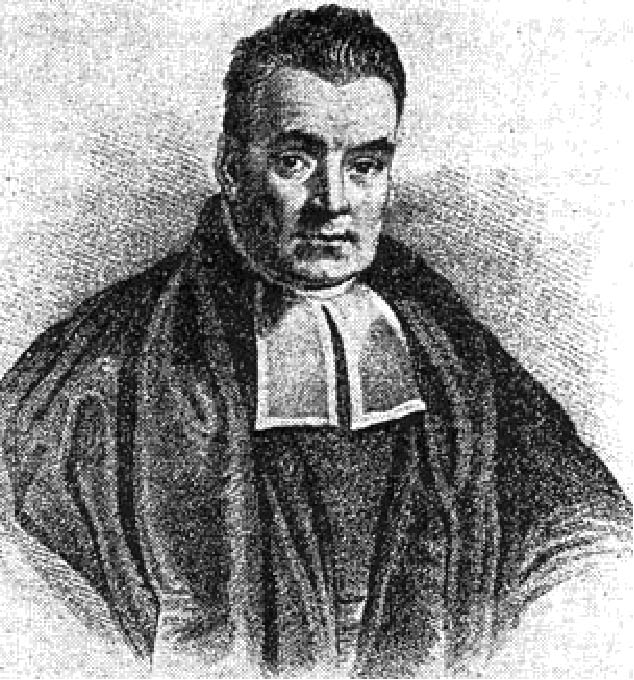
\includegraphics[width=0.4\textwidth,height=0.4\textheight]{Thomas_Bayes3.jpg}
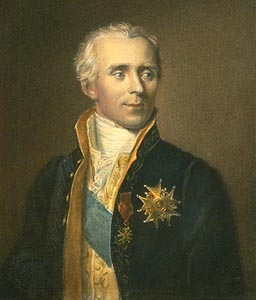
\includegraphics[width=0.4\textwidth,height=0.4\textheight]{Laplace.jpg}
\newline\tiny Thomas Bayes (1701--1761; left) and Pierre-Simon Laplace
(1749--1827; right)
\end{frame}

\begin{frame}{In practice}
\protect\hypertarget{in-practice}{}
\[\underbrace{P(\boldsymbol{\theta}|x)}_{\text{posterior}}\propto \overbrace{\mathcal{L}(x|\boldsymbol{\theta})}^{\text{Likelihood}}\underbrace{P(\boldsymbol{\theta})}_{\text{prior}}\]

\begin{itemize}
\tightlist
\item
  \(x\) is the observed data
\item
  \(\boldsymbol{\theta}\) are the parameters of interest
\item
  Note 1: \(P(x)\) is not tractable, but it is constant
\item
  Note 2: A uniform prior results in
  \(P(\boldsymbol{\theta}|x)\propto \mathcal{L}(x|\boldsymbol{\theta})\)
\end{itemize}
\end{frame}

\begin{frame}{Bayesian versus Frequentist}
\protect\hypertarget{bayesian-versus-frequentist}{}
\begin{block}{Bayesian:}
$$\hat{\boldsymbol{\theta}}_{\text{MAP}}=\underset{\boldsymbol{\theta}}{\text{argmax}}  \;P(\boldsymbol{\theta}|x)$$


\begin{itemize}
    \item The true parameter is treated as random.
    \item The estimate is chosen as the posterior mode.
\end{itemize}
\end{block}

\begin{block}{Frequentist:}
$$\hat{\boldsymbol{\theta}}_{\text{MLE}}=\underset{\boldsymbol{\theta}}{\text{argmax}} \;\mathcal{L}(x|\boldsymbol{\theta})$$
\begin{itemize}
    \item The true parameter is treated as constant.
    \item Estimate aims to maximize the probability of observing data.
\end{itemize}
\end{block}
\end{frame}

\begin{frame}{Benefits of Bayes over Frequentist}
\protect\hypertarget{benefits-of-bayes-over-frequentist}{}
\begin{itemize}
\tightlist
\item
  The ability to incorporate prior knowledge
\item
  More interpretable

  \begin{itemize}
  \tightlist
  \item
    Credible intervals vs.~confidence intervals
  \item
    Estimation of probability of hypotheses
  \item
    Resolves some of the limitations of p-values
  \end{itemize}
\item
  More flexible

  \begin{itemize}
  \tightlist
  \item
    Hierarchical models are more straightforward
  \item
    Easier to take measurement uncertainty into account
  \item
    Non-standard hypothesis testing by probing the posterior
  \end{itemize}
\end{itemize}
\end{frame}

\begin{frame}{Drawbacks of the Bayes approach:}
\protect\hypertarget{drawbacks-of-the-bayes-approach}{}
\begin{itemize}
\tightlist
\item
  Computationally complex \& demanding
\item
  Prior specification is very important

  \begin{itemize}
  \tightlist
  \item
    Too strong of a prior can bias results
  \item
    Can affect tractability (remedied by conjugate priors)
  \end{itemize}
\item
  Not what people are used to seeing
\end{itemize}
\end{frame}

\begin{frame}{NUTS}
\protect\hypertarget{nuts}{}
\begin{frame}
  \animategraphics[width=\textwidth]{12}{gif/frame-}{0}{39}
\end{frame}
\end{frame}

\end{document}
